\section{Real-world applications}\label{sec:Applications}
In this section, we illustrate the application of the above discussed methods on selected  examples from theory and real-world research questions. We focus on recurrence network approaches, (horizontal) visibility graphs, and transition network approaches, since those methods have found much wider and deeper applications in diverse fields.

	\subsection{Recurrence networks}
		Although recent work on RNs and multivariate generalizations thereof has been focused on the development of the theoretical framework and its numerical exploration using simple low-dimensional model systems, there have already been several successful applications to characterizing system's properties from experimental or observational time series. For example, the successful application of RN to predict protein structural classes has been reported in \cite{Olyaee2016}. Here we summarize some main applications to various disciplines and choose one successful application to understanding climate regularities.

		\paragraph{Applications in Earth sciences}
		One important field of recent applications is paleoclimatology, which has already been taken as an illustrative example in the seminal paper by Marwan \textit{et~al.} \cite{Marwan2009}. The corresponding study was later extended to a systematic investigation of the temporal variability profile of RN-based complexity measures for three marine sediment records of terrigenous dust flux off Africa during the last 5 million years. Donges \textit{et~al.} \cite{Donges2011,Donges2011a} argued that RNs can be used for characterizing dynamics from non-uniformly sampled or age-uncertain data, since this methodological approach does not make explicit use of time information. In turn, due to the necessity of using time-delay embedding, there is implicit time information entering the analysis, which has been recognized but widely neglected in previous works. Notably, disregarding age uncertainty and sampling heterogeneity appears a reasonable approximation only in cases where the distribution of instantaneous sampling rates remains acceptably narrow. In fact, more recent findings point to a strong dependence of the validity and robustness of the results obtained for paleoclimate time series on the specific archive and proxy variable \cite{Lekscha2018}. As an alternative, the letter study suggested utilizing derivative embedding instead of time delay embedding for phase space reconstruction and discussed several approaches for numerically estimating the numerical derivatives of the time series values required for this procedure. Another approach for tackling the problem of potentially non-robust individual significance of RN properties for individual time series integrates information from multiple paleoclimate time series and explicitly propagates age uncertainty to RN-measure uncertainties. This multi-archive approach has been used to investigate non-linear regime shifts in Asian summer monsoon variability during the Holocene and its potential impacts on human societies, conflicts and migration \cite{donges2015nonlinear}.

		As another methodological step towards better understanding climatic mechanisms, Feldhoff {\textit{et al.}} have used two speleothem records for studying interdependencies between the two main branches of the Asian summer monsoon (the Indian and East Asian summer monsoon) by means of inter-system recurrence network (IRN) approaches \cite{Feldhoff2012,Marwan2012Nolta}. For this purpose, they selected two data sets of oxygen isotope anomalies from speleothems obtained from two caves in China and the Oman, respectively, which can be considered as proxies for the annual precipitation and, hence, the overall strength of the two monsoon branches over the last about 10,000 years. The asymmetries of the IRN cross-transitivities and global cross-clustering coefficients provided clear evidence for a marked influence of the Indian summer monsoon on the East Asian branch rather than vice versa, which is in good agreement with existing climatological theories. As a subsequent extension of this work, Feldhoff {\textit{et al.}} emphasized the possibility of repeating the same kind of analysis in a sliding windows framework, thereby gaining information on possible temporal changes of the associated climatic patterns during certain time periods as recently revealed using correlation-based complex network analysis applied to a larger set of speleothem records from the Asian monsoon domain \cite{Rehfeld2012}.

		In order to characterize dynamical complexity associated with more recent environmental variability, Lange and B\"ose \cite{Boese2012,Lange2013Book} used RQA as well as RN analysis for studying global photosynthetic activity from remote sensing data in conjunction with global precipitation patterns. Specifically, they studied 14-years long time series (1998-2011) of the fraction of absorbed photosynthetically active radiation with a spatial resolution of 0.5$\degree$ around the Earth and a temporal sampling of about ten days, providing time series of $N=504$ data points. Their results revealed very interesting spatial complexity patterns, which have been largely, but not exclusively determined by the amplitude of the annual cycle of vegetation growth in different ecosystems.

Finally, RN analysis -- in combination with more traditional RQA characteristics -- has been employed recently for studying temporal variations in the dynamical complexity of geomagnetic field fluctuations at time-scales between hours and weeks associated with sequences of quite-time magnetic field episodes and geomagnetic storms \cite{Donner2018}. It has been shown that especially the RN transitivity allows a unique discrimination between the corresponding ``physiological'' and ``pathological'' states of the Earth's magnetosphere. A follow-up work investigated the corresponding changes in RN and RQA characteristics in greater detail for the same geomagnetic activity index (Dst) together with corresponding changes in solar wind variables that could particularly affect the stability of the Earth's magnetic field \cite{Donner2018b}.

		\paragraph{Applications in fluid dynamics}
		In a series of papers, Gao \textit{et~al.} investigated the emerging complexity of dynamical patterns in two-phase gas-liquid or oil-water flows in different configurations using RN techniques. Bifurcation scenarios from slugs to bubbles of a two phase flow of water-air occurring in a circular horizontal mini-channel have been recently analyzed by RPs and RN approaches in \cite{Gorski2015}. Similarly, the RN transitivity of pressure drop fluctuation time series has been used to distinguish between different dynamical patterns in two-phase flows \cite{Mosdorf2015}. In general, multiple sensors measuring fluctuations of electrical conductance have been used for obtaining signals that are characteristic for the different flow patterns. For gas-liquid two-phase upward flows in vertical pipes, different types of complex networks generated from observational data have been proposed, among which the degree correlations (assortativity) of RNs was proven to be particularly useful for distinguishing between qualitatively different flow types \cite{Gao2009,Gao2009a,Gao2010a}. One may also construct a directed weighted RN \cite{Gao2012,Gao2012a,Gao2013b,Gao2013d,Zhang2013b}. For oil-water two-phase upward flows in a similar configuration, the global clustering coefficient of RNs reveals a marked increase in dynamical complexity (detectable in terms of a decreasing $\hat{\mathcal{C}}$) as the flow pattern changes from slug flow over coarse to very finely dispersed bubble flow \cite{Gao2013,Gao2013c}. In case of oil-water two-phase flows in inclined pipes \cite{Gao2010}, the motif distributions of RNs (specifically, the frequency distributions of small subgraphs containing exactly four vertices) revealed an increasing degree of heterogeneity, where the motif ranking was conserved in all experimental conditions, whereas the absolute motif frequency dramatically changed. The corresponding results were independently confirmed using some classical measures of complexity, which indicated increasing complexity in conjunction with increasing heterogeneity of the RN motif distributions. Finally, for characterizing horizontal oil-water flows \cite{Gao2013,Gao2013d}, RN and inter-system RN analysis were combined for studying conductance signals from multiple sensors. Specifically, cross-transitivity was found a useful measure for tracing the transitions between stable stratified and unstable states associated with the formation of droplets. Furthermore, Gao {\textit{et al.}} \cite{Gao2015a,Gao2016,Gao2016b,Gao2016c} further extended these ideas to construct multivariate weighted recurrences networks from multi-channel measurements from different oil-water flow patterns.
        
        In a similar context, Charakopoulos \emph{et~al.} \cite{Charakopoulos2014} combined the $k$-nearest neighbor version of RNs and visibility graphs for studying temperature time series obtained from different parts of a turbulent heated jet, which allowed distinguishing dynamically different regions within the jet and attributing them to distinct physical mechanisms.

		\paragraph{Applications in electrochemistry}
		Zou \textit{et~al.} \cite{Zou2012b} studied the complexity of experimental electrochemical oscillations as one control parameter of the experiments (temperature) was systematically varied. By utilizing a multitude of complementary RN characteristics, they could demonstrate a systematic rise in dynamical complexity as temperature increased, but an absence of a previously speculated phase transition \cite{Wickramasinghe2010} separating phase-coherent from noncoherent chaotic oscillations. The latter results were independently confirmed using other classical indicators for phase coherence, as well as studies of a corresponding mathematical model of the specific electrochemical processes.

		\paragraph{Applications in medicine}
		Finally, there have been a couple of successful applications in a medical context. Marwan \textit{et~al.} \cite{Marwan2010c} demonstrated that the global clustering coefficients of RNs obtained from heartbeat intervals, diastolic and systolic blood pressure allowed a reliable identification of pregnant women with pre-eclampsia, a cardiovascular disease during pregnancy with a high risk of fetal and maternal morbidity. Their results were further improved by Ram\'{i}rez \textit{et~al.} \cite{Ramirez2012,Ramirez2013} who considered combinations of various RN-based network characteristics. In a similar spirit as for cardiovascular diseases, recent results point to the capability of RN characteristics for discriminating between the EEG signals of healthy and epileptic patients or to identify pre-seizure states in epilepsy patients \cite{Subramaniyam2013,Subramaniyam2015,ngamga2016,gao2018}.

		\paragraph{Understanding climate regularity transitions by RN analysis}
		The results of Donges \textit{et~al.}~\cite{Donges2011a} pointed to the existence of spatially coherent changes in the long-term variability of environmental conditions over Africa, which have probably influenced the evolution of human ancestor species. Specifically, RN transitivity and average path length have been interpreted as indicators for ``climate regularity'' (i.e., the complexity of fluctuations as captured by the transitivity dimensions) and ``abrupt dynamical changes'', respectively. By identifying three time intervals with consistent changes of the RN properties obtained from spatially widely separated records, it has been possible to attribute the corresponding long-term changes in the dynamics to periods characterized by known or speculated mechanisms for large-scale climate shifts such as changes in the Indian ocean circulation patterns, the intensification of the atmospheric Walker circulation, or changes in the dominant periodicity of Northern hemispheric glacial cycles. Moreover, Donges \textit{et~al.}\cite{Donges2011} demonstrated a good robustness of the results of RN analysis obtained in a sliding windows framework when varying the corresponding parameters (e.g., window size or embedding delay) over a reasonable range.

		More specifically, the paleoclimate variability transitions in East Africa have been demonstrated by analyzing marine sediment paleoclimate records from ocean drilling program (ODP) sites 659 in the East Atlantic, 721/722 in the Arabian Sea, and 967 in the Eastern Mediterranean Sea. The time series of three chosen sites are shown in Fig. \ref{fig:appl_recurrence_network}(a). To date, these marine sediments provide the only archive that allows the study of the Plio-Pleistocene African climate on all relevant time scales. However, earlier analyses of terrigenous dust flux records using traditional time series analysis techniques to detect important transitions in the African climate yielded partly contradictory results with respect to the signature and timing of these events \cite{deMenocal2004,Trauth2009}. Difficulties like these are to be expected when applying linear methods to the highly nonlinear climate system underlying paleoclimate proxy records. To circumvent this problem and explore the vast remainder of nonlinear phenomena, RNs can be used \cite{Donges2011a}.

		To this end, Donges \textit{et~al.} rely on two established measures of RNs: transitivity $\mathcal{T}$ and average path length $\mathcal{L}$. Furthermore, transitivity $\mathcal{T}$ has been interpreted as a climate regularity index since noisy or chaotic dynamics gives rise to low values, whereas (almost) periodic or laminar behavior induces high values. The average path length $\mathcal{L}$ shows much sensitivity on abrupt dynamical changes between different dynamical regimes when extreme values have been observed for $\mathcal{L}$. Both $\mathcal{T}$ and $\mathcal{L}$ together provide double-evidence points at a particularly relevant feature in the data since they are responsive to different nonlinear aspects of the time series data and do not necessarily show transitions at the same epochs.

		The results of $\mathcal{T}$ and $\mathcal{L}$ for the considered terrigenous dust record time series are shown in Fig. \ref{fig:appl_recurrence_network}(b, c). More specifically, $\mathcal{T}$ reveals surprisingly similar long-term change in short-term fluctuations before about 1.5 Ma B.P. (in contrast to the Mediterranean ODP site 967), although both sites are strongly geographically separated and, hence, characterized by distinct wind systems and dust sources (Fig.~\ref{fig:appl_recurrence_network}(b)). This overall picture indicates that changes in $\mathcal{T}$ during the Pliocene and early Pleistocene are robust manifestations of long-term variations in the dynamics of large-scale African dust mobilization and transport. More importantly, three transition periods can been identified which can be clearly related to distinct and known climatic mechanisms (Fig.~\ref{fig:appl_recurrence_network}) \cite{Donges2011a}.
		\begin{figure}[htbp]
		\centering
			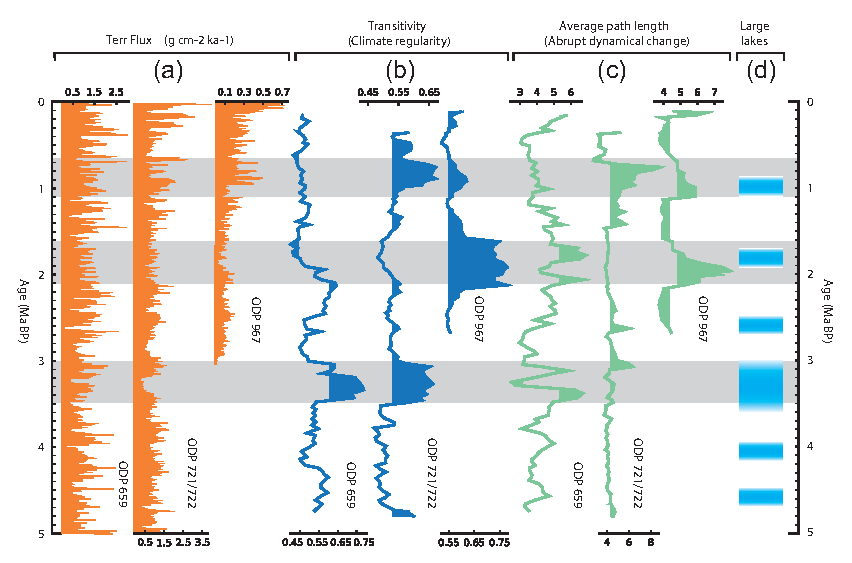
\includegraphics[width=\textwidth]{Chapter06_Applications/appl_recurrence_network.eps}
		\caption{(a) Terrestrial dust flux records from the three considered ODP sites distributed around Africa covering the Plio-Pleistocene. (b, c) Results of RN analysis of the three dust flux records including 90\% confidence (shading areas) of a stationarity test. Comparing both measures transitivity (interpreted as a measure of climate regularity) and average path length (interpreted as a measure of abrupt dynamical change in climate) for all records reveals significant and synchronous large-scale regime shifts in dust flux dynamics (horizontal shadings). (d) Time intervals with geological evidence for large lakes in East Africa, comprising collected information from different areas in the EARS and additional results from the Afar basin. Modified from \cite{Donges2011a}. } \label{fig:appl_recurrence_network}
		\end{figure}

		The first transition period is identified by a pronounced maximum of $\mathcal{T}$ between 3.5 and 3.0 Ma B.P. at both ODP sites 659 and 721/722 signaling a period of exceptionally regular dust flux dynamics (Fig.\ref{fig:appl_recurrence_network}(b)). The transition epochs highlighted by average path length $\mathcal{L}$ support these findings (Fig.~\ref{fig:appl_recurrence_network}(c)). The time interval 3.5 -- 3.0 Ma B.P. is characterized by three distinct and highly significant extrema (two maxima and one minimum in $\mathcal{L}$) in the ODP site 659 record, indicating shifts between regimes of higher and lower regularity in the variations of environmental conditions \cite{Donges2011a}. This identified long period during which global mean temperatures have been consistently higher than present day, which is thus considered as an analog for the future climate of the late 21st century if anthropogenic emissions of greenhouse gases continue to rise. At the same time, RN analysis reveals an enhanced $\mathcal{T}$ of African dust flux variations in both the Arabian Sea and Atlantic Ocean. At ODP site 721/722, this observation is predominantly caused by a well-pronounced epoch of relatively weak and approximately constant dust flux between about 3.36 and 3.17 Ma B.P. A similar --- but shorter --- feature is found at ODP site 659 between about 3.25 and 3.19 Ma B.P. (Fig. \ref{fig:appl_recurrence_network}(d)) as well as at ODP sites 661 and 662 in the Eastern Equatorial Atlantic. The presence of such very similar features with a clearly different timing suggests the presence of either one common climatological mechanism influencing the Arabian Peninsula much earlier than Northwest Africa or two distinct (but eventually interrelated) factors, where the first affected only the Northeast African and/or Arabian dust flux dynamics.

		The second identified transition is represented by an extended and highly significant maximum of $\mathcal{T}$ between about 2.25 and 1.6 Ma B.P. and of $\mathcal{L}$ between 2.2 and 1.7 Ma B.P. The latter one roughly coincides with the observations made at ODP site 659. The timing of this transition period in the Early Pleistocene (2.25 -- 1.6 Ma B.P.) well coincides with known large-scale changes in atmospheric circulation associated with an intensification and spatial shift of the Walker circulation.

		Moreover, the third transition period is between about 1.1 and 0.7 Ma B.P., when both $\mathcal{T}$ and $\mathcal{L}$ show significant maxima for ODP sites 967 and 721/722 but not for ODP site 659. This interval corresponds to the Middle Pleistocene transition (MPT) characterized by a change from glacial cycles predominantly related to obliquity variations of Earth's orbit (approximately 41 ka period) to such with an approximately 100 ka periodicity. The timing of this transition and its underlying mechanisms have been extensively studied elsewhere. That the MPT is not detected in the record from ODP site 659 by RN analysis does not imply that it did not have any climatic impact in the corresponding dust-source areas in Northwest Africa. Instead it shows that our technique is not sensitive to the local signature of the transition, if present, e.g., if it manifests itself in some change of trend \cite{Donges2011a}. Alternatively, the locally available data may be insufficient in quality and/or resolution to reveal the subtle type of events RN analysis is focusing on.

		In summary, this analysis identifies three main epochs of interest: 3.5 -- 3.0, 2.25 -- 1.6, and 1.1 -- 0.7 Ma B.P., as shown in Fig.\ref{fig:appl_recurrence_network}. All three are characterized by statistically significant extrema of $\mathcal{T}$ and/or $\mathcal{L}$ in at least two of the analyzed records. In addition, there are further shorter time periods of considerably increased or decreased $\mathcal{T}$ or $\mathcal{L}$ observed in the different records which coincide with environmental changes too (lake level high stands, Fig.~\ref{fig:appl_recurrence_network}(d)). Based on results from a meta-anaylsis using event coincidence analysis, tt was furthermore proposed that these detected large-scale changes in climate regularity may have acted as drivers of human evolution in Africa during the Plio-Pleistocene \cite{Donges2011a}.


	\subsection{Visibility graphs} \label{sec:appVGs}

	Very similar as RN approaches, (H)VGs have been applied to experimental time series from various fields, for instance, energy dissipation rates in fully developed turbulence \cite{Liu2010,Manshour2015,Manshour2015a}, financial data \cite{Ni2009,Yang2009,Qian2010,Wang2012,Flanagan2016}, physiological time series \cite{Lacasa2009,Shao2010,Dong2010,Ahmadlou2010,Jiang2013,Hou2014}, seizure detections by EEG signals \cite{Bhaduri2015,Liu2017a,Zhang2018}, cardiorespiratory interaction signals \cite{Long2014}, and alcoholism identification by EEG signals \cite{Zhu2014}. In the geoscientific context, \cite{Elsner2009} studied the time series of annual US landfalling hurricane counts. Subsequently, further studies investigated daily streamflow series from the US and China \cite{Tang2010}, air temperature data from China \cite{Wang2009}, wind speed records from central Argentina \cite{Pierini2012}. In the field of paleoclimatology, VG-based tests for time-reversal asymmetry were used to detect indications for a North Atlantic ocean circulation regime shift at the onset of the Little Ice Age \cite{schleussner2015indications}. VGs were also used for studying seismic activity in Italy \cite{Telesca2012}  and the  Corinth rift in western central Greece \cite{Hloupis2017}. Nonlinear features of seismic time series have been recently reviewed in \cite{Telesca2018b}. Both $k$ nearest neighbors network and VG analysis show almost the same qualitative behavior and allow to reveal the underlying system dynamics in turbulent heated jets \cite{Charakopoulos2014}. Furthermore, the VG approach has been used to disclose the fractal properties of the event-by-event fluctuations of multiparticle production in Nucleus-Nucleus collisions \cite{Mondal2018}.

	 Motif structures and subgraphs played important roles in forming VGs, which have been used to human ventricular fibrillation (ECG) time series \cite{Li2011,Li2012}, ECG diagnosis of epilepsy \cite{Tang2013}, and air traffic flow data \cite{Liu2018}. Simple topological measures such as the diameter, average path length, modularity, clustering coefficient, density and hierarchical organizations of networks have been used to characterize different dynamic properties between atmospheric and oceanic variables \cite{CHARAKOPOULOS2018}. In addition, the (H)VGs have been proposed to predict catastrophes of a non-autonomous network which derived from a marine system \cite{Zhang2018b}, which demonstrates that the topological characteristics like average degrees of the networks do show pronounced signatures at the onset of catastrophes. Fractal characteristics of (H)VGs have been reported in fractional Brownian motions, which has been recently extended to multiparticle emission data in high energy heavy-ion collisions \cite{Mali2018}, which shows consistent power law degree distributions as compared to the results as obtained by the traditional sandbox algorithm. In \cite{Gao2016}, a slight modification of HVG algorithm has been proposed to extract the multiscale properties of time series from oil-water two phase flow signals. In the case of intermittent time series, some phenomenology theories have been obtained in order to link the laminar episodes and chaotic bursts with the connectivity of the resulting HVGs \cite{Nunez2013,Nunez2014}.

		Next, we illustrate two specific examples showing the applications of (H)VG analysis to identify nonlinear ocean circulation regime shifts by paleoclimate time series of ocean sediment cores and time series of sunspots.

		\paragraph{VG analysis of nonlinear ocean circulation regime shifts at the onset of the Little Ice Age} \textit{Schleussner et al.} applied HVG-based tests for time-reversal asymmetry to paleoclimate records to detect indications for a North Atlantic ocean circulation regime shift at the onset of the Little Ice Age \cite{schleussner2015indications}.

		The transition from the Medieval Climate Anomaly (MCA) to the Little Ice Age (LIA) primarily in the  Northern Hemisphere is one of the most important climatic shifts during the pre-industrial last millennium. Although recent paleoclimatic reconstructions reveal no coherent global-scale cooling at the onset of the LIA, they agree on a generally colder period from the 16th to the 19th century (e.g. \cite{Pages2K2013}). Alternatively, \textit{Masson-Delmotte et al.} \cite{IPCC_AR5_WG5_Ch5} give a period between 1450 and 1850. In Europe, the regional expression of the LIA is associated with a spatially and temporally heterogeneous cooling, being most pronounced in central and northern Europe \cite{buentgen_tegel11,Pages2K2013}.

		Besides uncertainties in timing and extent, also the origin of this climate shift is still a subject of debate. Since the LIA coincides with several minima in the total solar irridiance (TSI), solar activity has been proposed as a possible driver already by \textit{Eddy et al.}\cite{eddy76}. The impact of TSI changes on the coupled ocean-atmosphere system in the North Atlantic has been investigated in a variety of different model studies \cite{crowley00,zorita_storch04,swingedouw_terray12}. As an alternative hypothesis, volcanic eruptions have been suggested as the origin of the regional cooling \cite{robock79,crowley00}. Despite the short life-time of volcanic aerosol loadings, they have been found to influence North Atlantic climate variability on multi-decadal time scales \cite{ottera_bentsen10,fischer_luterbacher07,zanchettin_timmreck11,goosse_crespin12}. Decadally-paced volcanic eruptions have been reported to trigger coupled sea-ice oceanic feedbacks leading to a sustained slow-down of the Atlantic Meridional Overturning Circulation (AMOC) and persistent hemispheric cooling in modelling studies of the last millennium \cite{miller_geirsdottir12,schleussner_feulner13}.

		\textit{Schleussner et al.} \cite{schleussner2015indications} present additional evidence for such a non-linear regime shift in the North Atlantic circulation dynamics during the MCA-LIA transition based on an analysis of two fossil diatom based high-resolution August sea surface temperature series from two ocean sediment cores from the central subpolar basin (Rapid 21-COM) and the Norwegian Sea (CR 948/2011). They find robust signatures of time-irreversibility in both records during the MCA-LIA transition using a test based on horizontal visibility graphs. Comparison with simulations with the climate model of intermediate complexity CLIMBER-3$\alpha$ reveals good agreement between the sediment cores and model outcome. Paleo reconstructions as well as model results support the hypothesis of a non-linear oceanic regime shift at the onset of the LIA.

		Despite a basin-wide cooling in the whole North Atlantic, the Rapid 21-COM time series exhibits a warming during the LIA. On the contrary, CR 948/2011 shows an abrupt cooling after 1400, preceding the Rapid 21-COM warming by about 50 years (compare Fig.~\ref{fig:lia_vg_analysis} a (b) for CR 948/2011 (Rapid 21-COM)). A warming signal in the subpolar North Atlantic in contrast to a cooling in the Nordic Seas is also found in sub-decadal ocean sediment records from North Iceland and North East Newfoundland \cite{sicre_wekstroem14}. \textit{Andrews et al.}\cite{andrews_jennings14} report signatures of a major environmental shift at the MCA-LIA transition in two calcite and quartz based sediment records from the Denmark Strait.

		\textit{Schleussner et al.} perform a sliding window test for time series irreversibility as described above for the Rapid 21-COM as well as CR 948/2011 record over the pre-industrial last millennium from 1000 to 1800 AD (Fig. \ref{fig:lia_vg_analysis} c--f). Results for the degree and local clustering based tests are depicted in the middle and bottom panel for different window sizes. The window size is varied between 30 and 60 data points, which comprises between 240 and 480 years given an average sampling rate of 8 years for both cores. The choice of small window sizes comes at the cost of an increased rate of false positives \cite{Donges2013}, but allows to detect regime shifts that occur within time scales of a few decades.

		\begin{figure}
		\noindent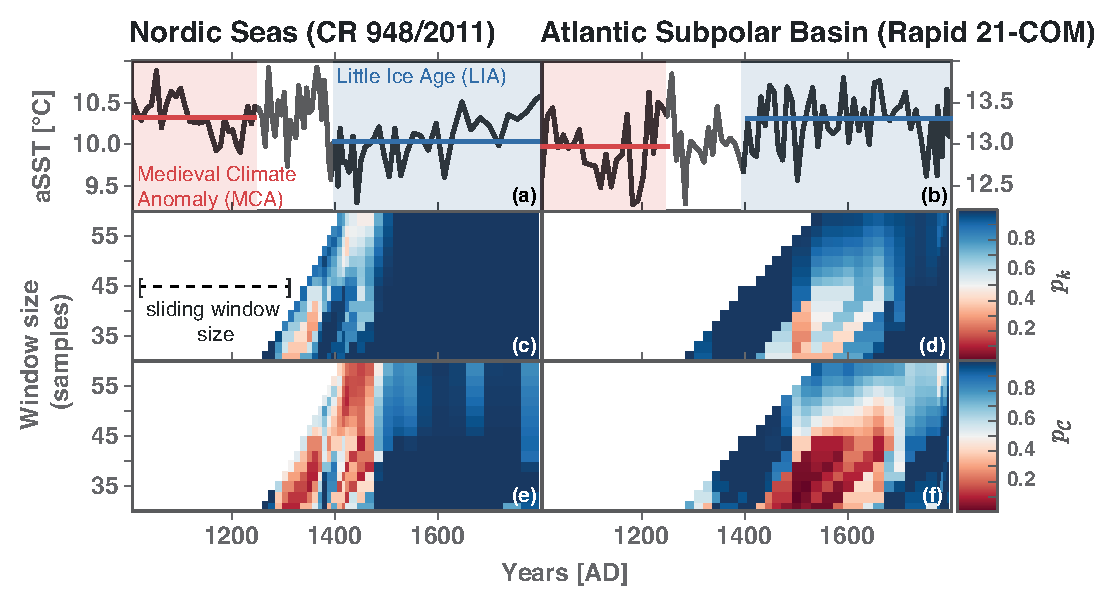
\includegraphics[width=\columnwidth]{Chapter06_Applications/schleussner_lia_vg_analysis.eps}
		\caption{Results of sliding window HVG-based tests for time-series irreversibility to detect nonlinear regime shifts in Atlantic paleooceanic dynamics during the past millennium. Reconstructed aSST time series from (a) the Nordic Seas (CR 948/2011) and (b) the Atlantic subpolar basin (Rapid 21-COM). The MCA (until 1250) and the LIA period (1400--1850) are shaded in red and blue, respectively, and the means over the MCA and LIA periods are depicted by solid lines coloured accordingly. (c, d) Results of the degree - based HVG time series irreversibility tests ($p_k$) for different window sizes. $p$-values close to unity (blue) indicate full reversibility, whereas close to zero (red) point towards time-irreversibility. (e, f)) Results of the clustering - based HVG time-irreversibility tests ($p_\mathcal{C}$). Figure modified from \cite{schleussner2015indications}.}
		\label{fig:lia_vg_analysis}
		\end{figure}

		The authors detect a clear signature of time-irreversibility using the clustering based test with $p$-values $p_C < 0.05$ for Rapid 21-COM and window sizes below 45 data points between 1450 and 1550 and $p_C \leq 0.1$ for CR 948/2011 and all window sizes around 1400 (see Fig. \ref{fig:lia_vg_analysis}, e,f). The $p$-values for the degree based test are somewhat higher (about 0.2, see Fig. \ref{fig:lia_vg_analysis}, c, d), which shows that the degree based test alone does not imply a rejection of the NH at a high significance level. Still, the timing of the signatures of NH rejection for the degree based test matches very well with the clustering based test, thus giving additional confidence in the results.


		\paragraph{VG analysis for sunspot numbers} \label{subsec:sunnum}
		Solar activity is characterized by complex dynamics, showing the famous 11 years cycle. Zou {\textit{et al.}} \cite{Zou2014a} performed the VGs analysis on both the daily and monthly sunspot series. The natural VGs focus on the effects of the local maxima on the resulting graphs. In the particular case of sunspot series, local minima play important roles in forming the increasing and decreasing phases of the solar cycles. In order to disclose the contributions of local minima to the VGs, they proposed two ways to construct the network: one is from the original observable measurements and the other is from a negative-inverse-transformed series.

		More specifically, let us discuss the results of VGs for the International Sunspot Number (ISN)~\cite{sidcDataBelgium} (see \cite{Zou2014a} for more consistent results that are based on the sunspot area series). The VG analysis have been performed for both monthly and daily sunspot series, which yields, respectively, month-to-month and day-to-day correlation patterns of the sunspot activities. The degree sequence $k_i = \sum_j A_{i,j}$ and its distribution $p(k)$ reflects the maximal visibility of the corresponding observation in comparison with its neighbors in the time series. In the case of sunspot time series,
the contributions of local minimum values to the network is of interest -- something that has been largely overlooked by the traditional VGs. One simple solution is to study the negatively inverted counterpart of the original time series, namely, $-x(t_i)$, which quantifies the properties of the local minima. Therefore, we use $k_{-x}$ and $p(k_{-x})$ to denote the case of $-x(t_i)$. This simple inversion of the time series allows us to create an entirely different complex network.

		Figure~\ref{sn_sa_data}(a,b) show $p(k)$ of the VGs derived from the ISN series $\{x_i\}$ with heavy-tails corresponding to hubs of the graph, which clearly deviates from Gaussian properties. In contrast, $p(k^{-x})$ of the negatively inverted sunspot series $\{-x_i\}$ shows a completely different distribution, consisting of a bimodal property (Fig.~\ref{sn_sa_data}c,d), extra large degrees are at least two orders of magnitude larger than most of the vertices (Fig.~\ref{sn_sa_data}(d)).
		\begin{figure}
  		\centering
			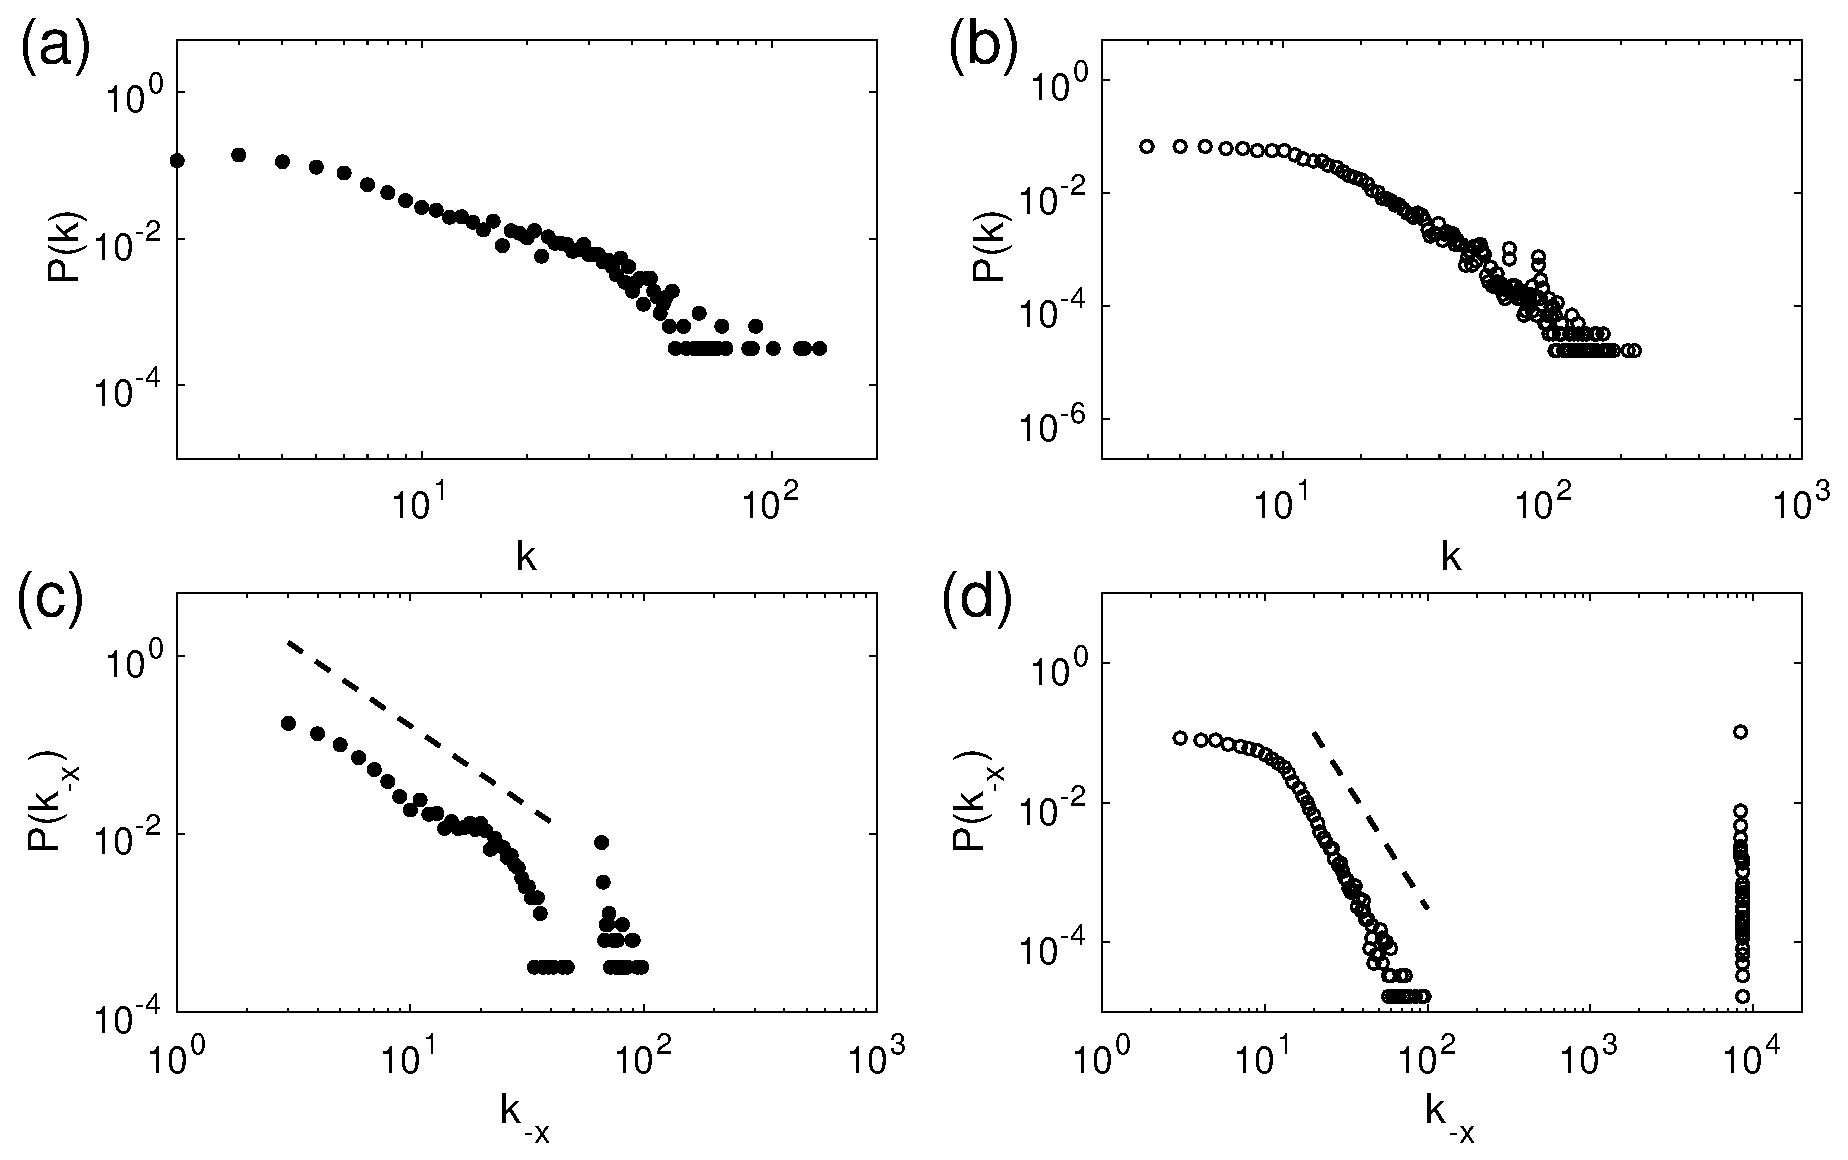
\includegraphics[width=0.8\columnwidth]{Chapter06_Applications/pdf_degreeBelgimN.eps}
		\caption{$p(k)$ of VGs from monthly (a,c) and daily data (b,d). (a,b) is for $\{x_i\}$, and (c,d) $\{-x_i\}$. One would suspect a fit to the first part of $p(k^{-x})$ yields that the slope of dashed line in (c) is 1.79, and that of (d) is 3.61, {\emph{but}} all $p$-values are $0$, rejecting the hypothetical power laws. Modified from \cite{Zou2014a}. } \label{sn_sa_data}
		\end{figure}
		Since well-defined scaling regimes are absent in either $p(k)$ or $p(k^{-x})$ (nor do they appear in the cumulative distributions, see more details of the statistical tests in \cite{Zou2014a}), the hypothesis of power laws is rejected.

		Based on the degree sequences $k_x$ and $k_{-x}$, we further investigate the long term variations of local maxima/minima of the sunspot series. We find that the positions of strong maxima are largely homogeneously distributed over the time domain, while that of the strong minima are much more clustered in the time axis. These results of the difference between maxima and minima could be used for evaluating models for solar activity because they reflect important properties that are not included in other measures reported in the literature. Furthermore, VGs for sunspot series show rich community structures, each of which mainly consists of the temporal information of two consecutive solar cycles. The solar cycle of approximately 11-years yields that most of the temporal points of the decreasing phase of one solar cycle are connected to those points of the increasing phase of the next cycle in the resulting VGs \cite{Zou2014a}. When the sunspot number reaches a stronger but more infrequent extreme maximum, we have inter-community connections, since they have a better visibility contact with more neighbors than other time points -- hence, forming hubs in the graph. The inter-community connections extend over several consecutive solar cycles encompassing the temporal cycle-to-cycle information. In Fig.~\ref{year_sspnDegBet}(a), some hubs of large degrees ($k_i > 15$) are highlighted, which have been suggested to identify solar cycles~\cite{Zou2014a}. In addition, there are strong positive correlations between large degrees $k_i$ and high betweenness $b_i$, which further characterizes the node's ability to transport information from one place to another along the shortest path (Fig.~\ref{year_sspnDegBet}(b)).
		\begin{figure}[htbp]
  		\centering
   			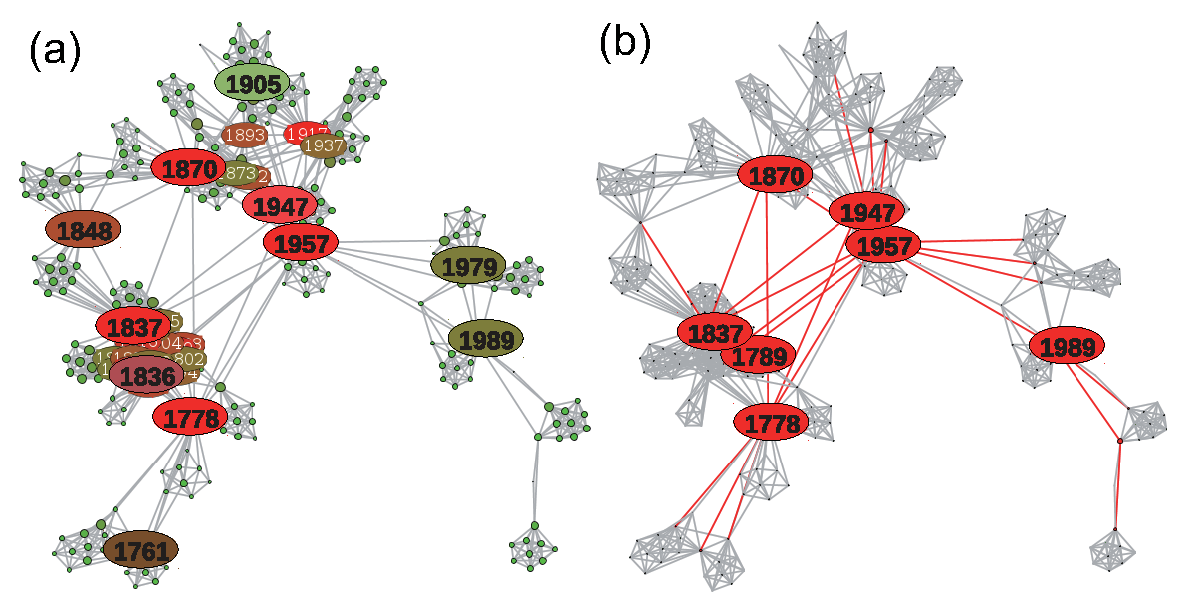
\includegraphics[width=\columnwidth]{Chapter06_Applications/network261_degree_between.eps}
			\caption{Network representations of the VG constructed from the annual sunspot numbers of the entire series. Highlighted visible nodes are: (A) large degrees ($k_i>15$), and (B) high betweenness centrality ($b_i>0.2$). Modified from \cite{Zou2014a}. } \label{year_sspnDegBet}
		\end{figure}


		\paragraph{Asymmetry of sunspots} \label{subsec:sunspotsAsym}
		Another important feature of sunspots is the presence of a marked, time-varying hemispheric asymmetry, which have not yet been completely resolved \cite{Newton1955,zolotova2009,donner2007}. The hemispheric asymmetry of solar activity manifests itself in the statistical properties of a variety of activity indicators such as sunspot numbers, areas and spatial distribution, the numbers of flares and coronal mass ejections, solar radio and X-ray flux, etc., and has been recognized to vary on multi-decadal time scales (see, e.g.,\cite{Newton1955,Carbonell1993,zolotova2006,donner2007,donner2008a,Li2008MNRAS,li2008a,zolotova2009}, and references therein). Notably, it is commonly believed that the observed distinct hemispheric asymmetry is an intrinsic property associated with the underlying solar magnetic field dynamics, which in turn serves as the driver of solar activity responsible for particle and electromagnetic emissions directly affecting the Earth. However, even despite these methodological advances, properly quantifying the North--South asymmetry is a challenging problem by itself. Specifically, the complex dynamics of the entire solar activity cycles calls for replacing traditional linear statistical approaches by methods originated in the field of nonlinear dynamics \cite{zolotova2006,donner2007}. In \cite{Zou2014}, Zou {\textit{et~al.}} proposed (H)VGs analysis to study the asymmetric distributions of the sunspots over the solar surface. They have argued that (H)VGs provide complementary information on hemispheric asymmetries in dynamical properties.

		More specifically as we discussed in Sec.\ref{subsec:jointdegreeVG}, the excess degree $\Delta k(t)$ (Eq. \eqref{eq:deltaK}) and the relative excess degree $\Delta_{rel} k(t)$ (Eq. \eqref{eq:deltaReK}) have been proposed to characterize the possible asymmetric properties for (H)VGs that are reconstructed from bivariate time series, which are resulted from two interacting layers $\alpha$ and $\beta$. These two measures are based on the computations of joint degree $k^{joint}(t)$ (Eq. \ref{eq:jointK}) and the conditional degree sequences $k_{{[\alpha]}, {[\beta]}}^{O}(t)$ (Eq. \ref{eq:nad}). We emphasize that the absolute excess degree can be easily interpreted in terms of inter-hemispheric differences, whereas the relative excess degree partially corrects for the skewness effect and allows quantitatively assessing the relevance of differences between the degree sequences of both hemispheres. When analyzing sunspot time series, it has been demonstrated in \cite{Zou2014} that absolute and relative excess degrees exhibit qualitatively the same long-term variability. Therefore, we review some results based on $\Delta k(t)$ only and further results of $\Delta_{rel} k(t)$ can be found in \cite{Zou2014}.

		First we construct the (H)VGs for monthly hemispheric sunspot area series $A_{N}(t)$ and $A_{S}(t)$, yielding the degree sequences $k_\mathrm{N}(t)$ and $k_\mathrm{S}(t)$, respectively. The long-term asymmetric distribution behavior of the sunspots has been captured by utilizing a sliding window technique that averages the degree sequence over some time period. In all following considerations the window size has been chosen as $w = 270$ months, with a mutual overlap of 12 months between subsequent time windows. This specific choice of the window size covers about one full period of the solar magnetic field polarity cycle (approximately 22 years). There are no marked changes in the long-term variability of the (H)VG-based characteristics for $w$ being between about 180 and 400 months.
\begin{figure}[htbp]
	\centering
	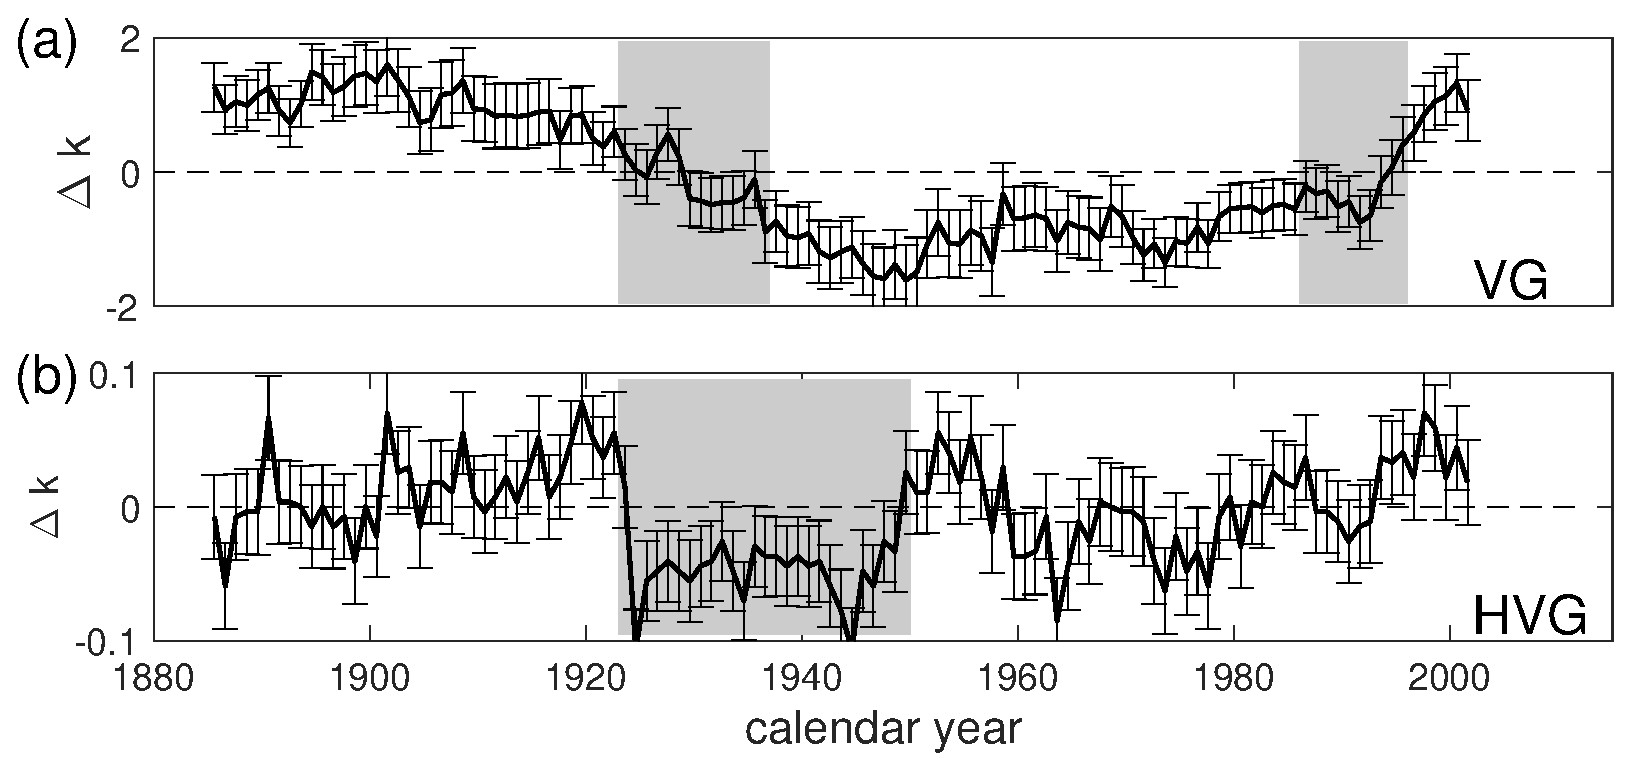
\includegraphics[width=0.8\columnwidth]{Chapter06_Applications/north_southDegreeComXWin130P.eps}
\caption{\small {(a) Absolute excess degrees $\Delta k_i$ obtained from the VGs of $A^{N,S}$ computed over the sliding windows with a width of $w = 270$ months and a mutual overlap of $12$ months. Error bars display mean values and standard deviations within a given time window centered at the respective point in time. Gray areas mark those time intervals where the sign of the excess degree changes. (b) $\Delta k_i$ from HVG. Reproduced from \cite{Zou2014}. }
\label{degreeComX_ns_area270}}
\end{figure}

		Figure~\ref{degreeComX_ns_area270} shows the mean features associated with the degree sequences for our sliding windows, together with the associated window-wise standard deviations. In the VG analysis (Fig.~\ref{degreeComX_ns_area270}(a)), our results reveal two transitions between periods of positive and negative mean absolute excess degrees, which take place at about 1925--1935 (from higher degrees in the Northern Hemisphere to those in the Southern one) and 1985--1995 (vice versa). Furthermore, positive (negative) excess degrees imply higher mean degrees in the Northern (Southern) Hemisphere. These observations have been partially explained by the strong asymmetry of the probability distributions of sunspots over the north and south hemispheres, for instance, very high positive skewness \cite{Zou2014}. The corresponding analysis by mean of HVGs (Fig.~\ref{degreeComX_ns_area270}(b)) reveals some interesting facts: first of all, all degree-related quantities obey considerably lower values and weaker overall variability than for the VG. This is to be expected since the HVG is a subgraph of the VG. However, while the absolute degree values in the HVG typically reduce by a factor of about 2--4 in comparison with the VG, the absolute excess degrees are by more than one order of magnitude smaller (Fig.~\ref{degreeComX_ns_area270}(b)).

		Moreover, for the HVG-based excess degree $\Delta k_i$ we do not find comparably clear indications for transitions between time periods with clear hemispheric predominance as for the VG (Fig.~\ref{degreeComX_ns_area270}(a)). The only notable exception is the time period between about 1925 (corresponding to the formerly identified first transition in the VG) and 1950, where the excess degree of the HVG is significantly negative (as also observed before for the VG). Specifically, the transition in the hemispheric predominance reflected by the VGs' conditional degree sequences coincides with a sharp drop in the corresponding series for the HVG at about 1925, whereas the end of the period of significantly negative excess degrees in the HVG at about 1950 accompanies the termination of the gradual downward trend of the excess degree obtained from the VGs (Fig.~\ref{degreeComX_ns_area270}(b)). Taken together, we interpret these findings such that the effect of the asymmetry of the hemispheric sunspot area values mostly dominates possible variations in dynamical characteristics. However, to this end we tentatively conclude that parts of the observed long-term changes of the VG-based excess degree cannot be explained by combining the corresponding changes in skewness and HVG-based excess degree (i.e., distribution and dynamics, respectively). One possible reason for this could be complex changes in the PDF of the sunspot areas, which go beyond fluctuations in skewness, but yet have a significant effect on the resulting VGs' properties.

		In summary, we conclude that temporal changes in the hemispheric predominance of the graph properties lag those directly associated with the total hemispheric sunspot areas. These findings open a new dynamical perspective on studying the North--South sunspot asymmetry, which needs to be further explored in future work.


	\subsection{Transition networks}
	Depending on the particular symbolic representations of time series, there are various applications of transition network approaches to real time series. For instance, co-movement time series of economic growth and high-end talent development efficiency \cite{Zhang2018b}. Here we focus on the application of ordinal pattern transition network approach as proposed by McCullough {\textit{et al.}} in \cite{McCullough2015}, where they applied this analysis to experimental time series generated by a diode resonator circuits. They argue that the network size, mean shortest path length, and network diameter are highly sensitive to the interior crisis captured in this particular data set. Meanwhile, the ordinal pattern partition networks have been reconstruct from Electrocardiogram (ECG) data from patients with a variety of heart conditions \cite{Kulp2016b}. Network measures of mean degrees, entropies of the set of ordinal patterns and the number of non-occurring ordinal patterns have been computed for the resulting transition networks, showing statistically significant difference between healthy patients and several groups of unhealthy patients with varying heart conditions.


	\paragraph{Ordinal pattern networks for externally driven diode resonator circuit}
	In \cite{McCullough2015}, McCullough {\textit{et al.}} constructed ordinal pattern transition networks for experimental time series from an externally driven diode resonator circuit. In this experiment, each time series of the circuit output voltage $U_R$ were recorded for evenly spaced values, which consists of 65536 observations. The amplitude of the driving sinusoidal voltage $U_0$ serves as a control parameter. When this control parameter $U_0$  is changed systematically in the range of $3V \leq U_0 \leq 5V$, the system presents rich bifurcation scenarios from periodic to chaotic dynamics. Our motivation of this example is to show that structural measures of the reconstructed ordinal pattern transition networks can track different routes to chaos. More visualizations of attractors in the corresponding phase space and their associated ordinal networks have been well demonstrated in \cite{McCullough2015}. In addition, we focus on three main network measures, the mean out-degree $\left < k_{out} \right >$, the mean shortest path length $\mathcal{L}$ and network diameter $\mathcal{D}$ (maximum shortest path length).
	\begin{figure}
	\centering
		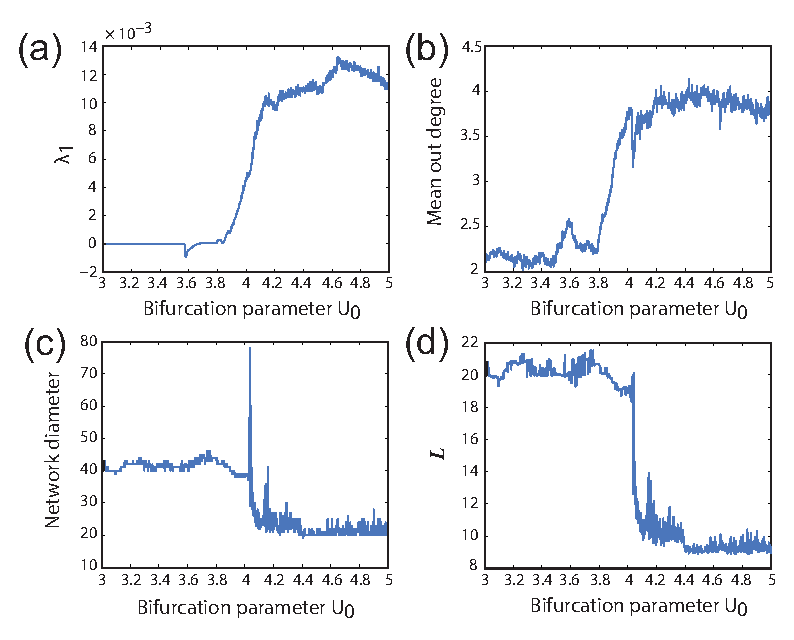
\includegraphics[width=0.8\columnwidth]{Chapter06_Applications/appl_transition_network.eps}
	\caption{Bifurcation diagram of the diode resonator data which are characterized by (a) the largest Lyapunov exponent $\lambda_1$ for the range $3V \leq U_0 \leq 5V$, (b) the mean out degree, (c) network diameter, and (d) mean shortest path length. Networks were generated for each time series with $\tau = 8$ and $D=8$. Modified from \cite{McCullough2015} with permission by AIP Publishing. } \label{fig:appl_transition_network}
	\end{figure}

	The full bifurcation spectrum of the data set is characterized by the largest Lyapunov exponent $\lambda_1$ and network measures (Fig.~\ref{fig:appl_transition_network}). The system begins in period-3 oscillations and undergoes a period doubling bifurcation into period-6 when the control parameter approaches $U_0 \approx 3.6$. The period doubling cascade to chaos is observed for the control parameter approximately $0.38 \leq U_0 \leq 0.405$, and further undergoes a step change at the interior crisis, reflecting the filling of the attractor. Each ordinal network is generated for each time series with $\tau = 8$ and $D = 8$. The period-3 and period-6 time series are mapped to ring structures. The network measures capture the bifurcation scenarios successfully (Figs.\ref{fig:appl_transition_network}(b-d)).

	More specifically, the periodic regime is captured by zero Lyapunov exponent $\lambda_1$. Note that $\lambda_1$ is computed by the {\tt{lyapk}} function of the TISEAN package \cite{kantz1997}. The small range of the control parameter $U_0$ for which $\lambda_1$ becomes negative around the first period doubling bifurcation is a numeric error due to poor parameter selection for those particular corresponding time series \cite{McCullough2015}. The size of the network exhibits sensitivity to both the period doubling bifurcation at $U_0 =3.6$, the period doubling cascade to chaos for approximately $0.38 \leq U_0 \leq 0.405$, and undergoes a step change at the interior crisis, reflecting the filling of the attractor. Furthermore, the mean out-degree $\left < k_{out} \right>$ provides robust tracking of dynamical change similar to $\lambda_1$, and also appear sensitive to the period doubling bifurcation and the interior crisis. The mean shortest path length $\mathcal{L}$ and network diameter $\mathcal{D}$ both undergo a clearly discernible step change at the interior crisis, with the latter also exhibiting a peak value at the change point. Both of these results are easily understood in terms of the relationship between the networks and phase space as follows: additional nodes and edges are created immediately after the crisis, corresponding to the intermittent chaotic trajectories that begin to fill the space between the bands of the pre-crisis attractor in phase space. These new nodes and edges become shortcuts in the network. The spike in diameter corresponds to the small number of time series which have only a limited number of trajectories in between the bands of the pre-crisis attractor because they are in the immediate vicinity of the crisis and we are dealing with finite non-stationary data. These trajectories will form new strands in the network which are only connected to the main structure where they leave and rejoin the bands of the pre-crisis attractor, and hence these trajectories will have a significant impact on the network diameter. Moreover, these strands or subgraphs will have a far lower degree and degree variance than the remainder of the network, hence why the value for mean out degree and degree variance also dips at the interior crisis.

	In summary, this set of results demonstrates that while $\left < k_{out} \right>$, mean shortest path length $\mathcal{L}$ and diameter $\mathcal{D}$ all share the deficiency that they do not provide an absolute criteria for discriminating between periodic and chaotic dynamics, they have the potential to be useful as an indicator for dynamical discrimination in a relative sense, and for detecting change points \cite{McCullough2015}.


	\paragraph{Ordinal pattern networks for electrocardiograms}
	In \cite{McCullough2017b}, McCullough {\textit{et al}} have introduced to compute both local and global out-link entropies of ordinal transition networks to quantify the complexity of temporal structure in the networks from time series. The numerical comparative investigation in the R\"ossler system has demonstrated that these complexity measures track dynamical changes through period doubling and periodic windows over a range of the bifurcation parameter. Furthermore, the analysis has been applied to time series of electrocardiograms (ECGs). More specifically, complexity measures are able to capture the unique properties, discriminating between short-time ECG recordings characterized by normal sinus rhythm (NSR), ventricular tachycardia (VT) and ventricular fibrillation (VF). The global node out-link entropy of each time series is computed for both a short and a long time embedding lag and the resulting two-dimensional vector constitutes a measure of multiscale complexity description.

	More specifically, the dataset comprises $81$ ECGs that were measured to observe different cardiac dynamics, including 31 records of NSR, 30 records of VT, and 20 records of VF \cite{McCullough2017b}. Each time series consists of $10000$ points in length and have been sampled at 500 Hz with 10 bits resolution. Then, the global node out-link entropy (Eq. \eqref{eq:globalTp}) has been used to quantify transitional complexity of the resulting ordinal pattern network which has been reconstructed for each ECG record.

	As we have discussed in Section \ref{sec:OPtransition}, the choice of embedding delay $\tau$ has certain effects on the resulting ordinal pattern networks. For the particular dataset of ECGs, McCullough {\textit{et al}} used a simple assumption that the mean resting heart rate is $80$ beats per minute, which is about 375 samples per cycle. Therefore, the short embedding lag is chosen as $\tau = 20$ which is approximately a quarter period of the complete cycle. Furthermore, a long embedding lag is chosen to be one order of magnitude larger $\tau = 200$ which will capture dynamics over segments of two to six cycles and encoding inter-cycle variability of the ECG in the resulting ordinal networks. The embedding dimension $m$ has been suggested as $5 \leq m \leq 10$. The transitional complexity $S^{GNE}$ has been computed for both a short and a long time embedding lag and the resulting two-dimensional figure constitutes a measure of multiscale complexity.
\begin{figure}[ht]
	\centering
	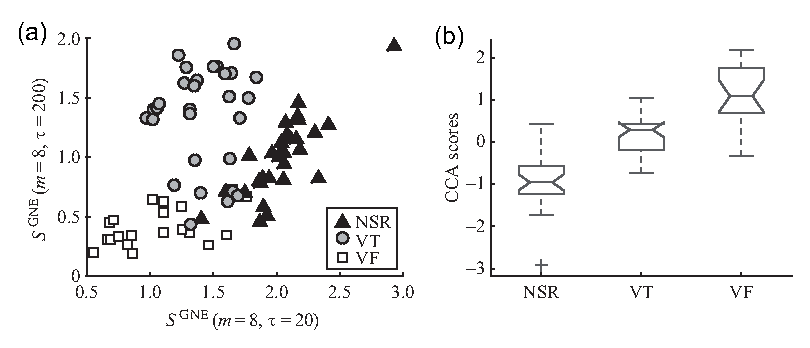
\includegraphics[width=\columnwidth]{Chapter06_Applications/RIE_CCU_ECG.eps}
\caption{(a) Scatter plot of global node out-link entropy $S^{GNE}$ for the $81$ ECG dataset. The $x$-and $y$-axes
correspond to $S^{GNE}$ computed with embedding $\tau =20$ and $\tau = 200$, respectively. (b) Box plot for the scores from a canonical correlation analysis of the data. Modified with permission from Ref. \cite{McCullough2017b}. Courtesy of M. Small. \label{fig:rieECG}}
\end{figure}

	Figure \ref{fig:rieECG} illustrates the two dimensional multiscale plot of $S^{GNE}$ and the corresponding box plot, which shows clear discrimination between the pathological groups. Therefore, ordinal networks present different level of transitional complexity corresponding to different networks.% The proper interpretation of actual values of $S^{GNE}$ in terms of dynamics for each group remains ambiguous. For instance, it appears to be counterintuitive that an ECG record for VF is apparently less complex than for NSR, which is however cannot be obtained from Fig. \ref{fig:rieECG}(a). This may be the effects of relative short length of time series \cite{McCullough2017b}.

		In addition, the ordinal network analysis is performed to characterize age-related effects in interbeat interval dynamics from ECGs. In \cite{McCullough2017b}, the authors further showed that the standard permutation entropy is unable to discriminate between age groups. In contrast, the global node out-link transitional complexity $S^{GNE}$ generally is higher for elderly subjects on short time scales and lower on long time scales, and $S^{GNE}$ has significantly greater variability than that can be observed for young subjects.
